\section{问题三：知识矩阵驱动的联合搜索与清除}
\subsection{状态表达与时间目标}
以频道为行、访问位置为列构造稀疏知识矩阵 $\mathsf M_t$。单元格状态包括未检测、无信号、示向、近距、清除失败和清除成功，附带真实坐标、角度与时间。沿行汇集同一目标的证据，沿列组织一次停点上的多频道检测。最终程序通过 \texttt{ChannelKnowledge} 将矩阵接入迭代调度，问题三入口为 \texttt{q3-v18}；独立的 \texttt{matrix} 策略作为对照路线。

路径列以120米量化建立索引，几何仍使用真实坐标。120米格既不是测向误差相同的区域，也不是光学定位精度；同格内两处测量不能视为重复读数。单元格保存摘要，连续测向历史由频道状态保存，动作日志用于完整复盘。失败清除摘要可能被同格后续反馈覆盖，这会减少可用负证据，不应将摘要表解释为全部历史。

记 $L$ 为路程、$N_s$ 为实际切频次数、$N_m$ 为检测次数、$N_o$ 为光学尝试次数、$N_c$ 为成功清除数，则
\begin{equation}
T=L/5+N_s+5N_m+3N_o+2N_c.\label{eq:time}
\end{equation}
清除失败只消耗3秒，成功共5秒，清除操作不切换测向频道。模型先要求全部清除，再优化 $T$；虚拟时间与真实程序运行时间分开统计。

\subsection{正负证据与保守可行域}
设 $\mathcal P_j,\mathcal N_j,\mathcal A_j,\mathcal F_j$ 分别为频道 $j$ 的示向、无信号、近距和清除失败记录。全向场景的精确位置约束可写为
\begin{equation}
K_j=\Omega\cap\bigcap_{i\in\mathcal P_j}(W_i\cap\disk(S_i,b))
\cap\bigcap_{i\in\mathcal A_j}\disk(S_i,5)
\setminus\left(\bigcup_{i\in\mathcal N_j}\disk(S_i,a)
\cup\bigcup_{q\in\mathcal F_j}\disk(q,20)\right).
\end{equation}
示向反馈还排除其检测点5米近距圆。减去圆盘通常得到非凸集合，最终实现将两种用途分开：用正观测构造含真值的凸多边形外包络 $\widehat K_j$，用于包围圆及覆盖清除认证；用全向无信号排除圆筛选区域样本，修正估计点，用于调度和试清。样本质心是启发式锚点，不能替代认证区域。

清除失败的20米排除圆通过矩阵传给覆盖计划，在整个方格都已确认无源时删去该格。全向无信号排除1000米、清除失败排除20米，两者作用范围和物理依据不同。只有 $\operatorname{dist}(S,\widehat K_j)>1500$ 才能安全跳过必然无信号的检测。

\subsection{发现层：圆心加六边形覆盖}
最终布局由圆心和半径1130米的正六边形顶点组成。对一般环半径 $r_h$、边数 $n$，目标圆最远点到最近扫描点的距离为
\begin{equation}
c_n(r_h)=\max\left\{\frac{r_h}{2\cos(\pi/n)},
\sqrt{R_0^2+r_h^2-2R_0r_h\cos(\pi/n)}\right\}.\label{eq:q3cover}
\end{equation}
证明见附录。代入 $n=6,r_h=1130$ 得覆盖半径约996.95米，小于接收半径下界1000米。因此完整执行各扫描点对未发现频道的检测，必能发现所有全向源。扫描点的访问顺序可改变，发现保证仅依赖点集与实际检测频道。

同一频道取得3条示向后，可停止后续扫描点的重复测向，转入清除任务；这一阈值只用于已发现目标，不能用于宣布未知频道不存在。检测时跳过已清除频道，近距反馈立即清除。
\begin{figure}[htbp]\centering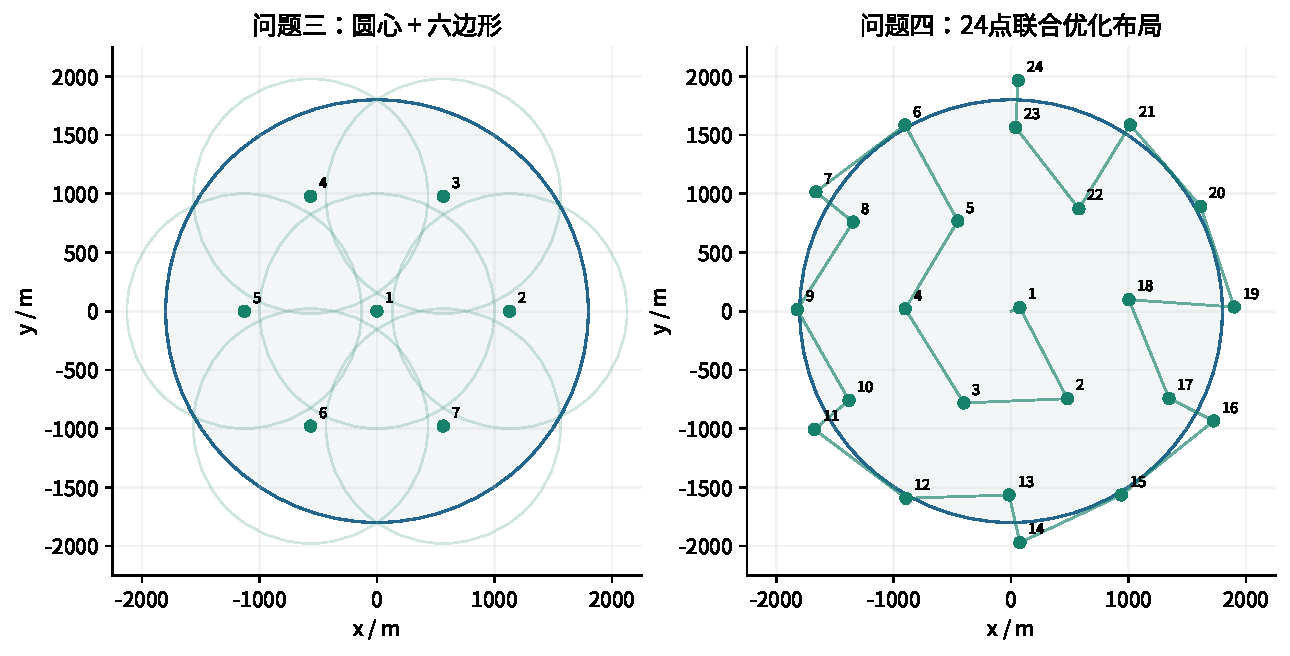
\includegraphics[width=.93\linewidth]{figures/layouts.pdf}
\caption{最终发现层布局：左为问题三七点布局，右为问题四24点布局及离线参考访问顺序。圆外扫描点符合题设移动范围。}\label{fig:layouts}\end{figure}

\subsection{扫描与清除任务联合调度}
固定“先扫描、再逐源清除”会重复经过相邻区域。为此构造动态任务集
\begin{equation}
\mathcal T_t=\{(\mathrm{scan},i,q_i):i\text{尚未访问}\}
\cup\{(\mathrm{clear},j,\widehat G_j):j\text{已发现且未清除}\}.
\end{equation}
只需一条有效读数即可生成目标锚点并登记清除任务。该任务会进一步测量或试清，并不意味着一条读数已经完成定位。

以当前位置为起点，用最近邻构造开放路线，再用2-opt反转片段消除绕行，最后用or-opt将连续1至3个任务搬移至其他位置，接受整条路线长度严格下降的候选，最多执行4轮or-opt。形式上求可行近似解
\begin{equation}
\min_\pi\left\{\norm{z_0-z_{\pi(1)}}+
\sum_{k=1}^{m-1}\norm{z_{\pi(k+1)}-z_{\pi(k)}}\right\},
\end{equation}
其中 $z_0$ 为当前位置。只执行路线首个任务，获得新反馈后重建任务集。这是滚动优化，所得路线是可行上界而非全局最优解；锚点变化使任务实际成本与静态路长不同。

\subsection{直接试清、补测与覆盖式清除}
到达估计点后先尝试光学清除。$r_*(\widehat K_j)>20$ 只表示不能保证该点覆盖全部可能位置，并不表示该点距真源必超过20米。因此以3秒失败代价换取直接命中的机会有实际价值。清除失败后先检查小规模覆盖计划，若不划算，再按问题二的交会原则补测；近共线情况下采用侧向候选。基类补测仍失败时启动覆盖兜底。

将平面划分为边长 $s=25$ 米的方格，格心记为 $z_C$，选择
\begin{equation}
\mathcal H_j=\{C:C\cap\widehat K_j\ne\varnothing\}.
\label{eq:coverclear}
\end{equation}
程序将格网原点对齐至可行域包围盒下界，通过顶点包含与边相交判定选出相交格，减少窄区域的冗余候选。若一个格的四个顶点均位于同一个失败清除圆内，则剔除该格。对其余格心依次试清，命中即停止。
\begin{proposition}
若 $G_j\in\widehat K_j$、清除反馈准确、所选格心均可达且计划完整执行，则覆盖式清除必能清除该目标。
\end{proposition}
\begin{proof}
真源所属方格 $C_G$ 满足 $\norm{z_{C_G}-G_j}\le25/\sqrt2\approx17.678<20$，因而必被选入。由范数凸性，四角均在失败排除圆内意味着整格在圆内，所以含真值的格不会被安全剔除。访问 $z_{C_G}$ 时必能清除目标。
\end{proof}

若计划有 $k$ 个点、全部访问路程为 $L_H$，成功前的最坏耗时上界为
\begin{equation}
T_H\le L_H/5+3k+2.\label{eq:clearcost}
\end{equation}
与“补测再清除”的参考成本 $L_m/5+10+\sigma$ 比较，其中 $\sigma\in\{0,1\}$ 表示是否切频。当前代码采用 $\sigma=1$ 的固定参考，且 $L_m$ 只估计到补测点的移动，所以这是动作选择代理，不是任意反馈下的严格最优判据。固定动作项在 $k=1,2$ 时为5、8秒，均小于10至11秒；$k=3$ 时为11秒，需要结合切频和路程判断。问题三前置计划最多2点，后置最多64点；超过上限时不截取不完整计划冒充覆盖。
\begin{figure}[htbp]\centering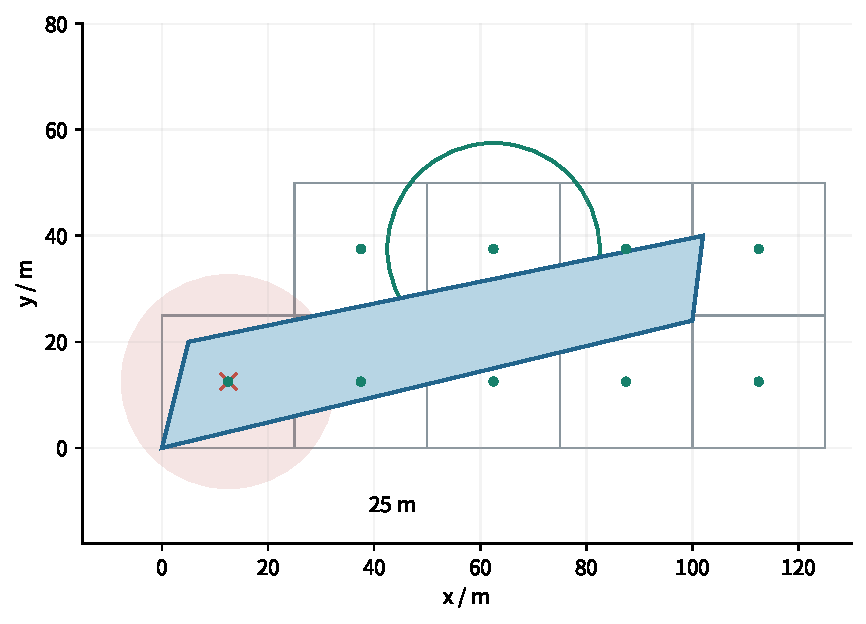
\includegraphics[width=.78\linewidth]{figures/cover_clear.pdf}
\caption{25米方格覆盖式清除示意。蓝色为保守可行域，红色圆为已失败的20米清除范围，绿色圆显示一个格心的有效清除范围。图为几何示意，非真实案例轨迹。}\end{figure}

\subsection{完整流程与保证边界}
\begin{enumerate}
\item 从原点、频道1初始化20个频道状态、知识矩阵及七点扫描任务。
\item 对待扫描点和已发现目标联合规划，每次执行首个任务，按实际反馈更新证据。
\item 执行直接试清、小规模覆盖计划、必要补测和后置覆盖计划，收到成功反馈才移除目标。
\item 扫描任务结束后处理仍未清除频道，核对未知频道的完整扫描记录。
\end{enumerate}
理论上的完成条件是已发现频道全部清除，且每个未发现频道满足
\begin{equation}
\Omega\subseteq\bigcup_{q\in\mathcal N_j}\disk(q,1000).\label{eq:certificate}
\end{equation}
不能以“已清除10个”或“待办队列为空”代替该条件。

上述发现覆盖和清除覆盖均为充分条件，但当前程序还含时间预算、调度重试次数、64格上限及退化区域分支。因此其完整性论证以这些条件未中断覆盖执行为前提，有限批实验的全清率不能提升为所有输入下的无条件保证。若仍有未清目标，需如实报告未完成。对单次示向的1500米长窄扇形，附录给出至多225格的理论兜底构造；该构造可说明有限光学覆盖的存在性，不冒充已接入的64格执行流程。
